\documentclass[journal]{IEEEtran}
\usepackage{amsmath,amsfonts}
% \usepackage{algorithmic}
\usepackage{algorithm}
\usepackage{algpseudocode} % For more flexible 
\usepackage{array}
% \usepackage[caption=false,font=normalsize,labelfont=sf,textfont=sf]{subfig}
\usepackage[]{subfig}
\usepackage{textcomp}
\usepackage{stfloats}
\usepackage{url}
\usepackage{verbatim}
\usepackage{graphicx}
% \usepackage{booktabs} % For professional-quality tables
\usepackage{cite}

\usepackage{makecell}   % 支持更灵活的单元格对齐和内容换行
\usepackage{multirow}
\usepackage{pifont}
\hyphenation{op-tical net-works semi-conduc-tor IEEE-Xplore}
% updated with editorial comments 8/9/2021


% -------------------------允许算法跨页-------------
\makeatletter
\newenvironment{breakablealgorithm}
  {% \begin{breakablealgorithm}
   \begin{center}
     \refstepcounter{algorithm}% New algorithm
     \hrule height.8pt depth0pt \kern2pt% \@fs@pre for \@fs@ruled
     \renewcommand{\caption}[2][\relax]{% Make a new \caption
       {\raggedright\textbf{\ALG@name~\thealgorithm} ##2\par}%
       \ifx\relax##1\relax % #1 is \relax
         \addcontentsline{loa}{algorithm}{\protect\numberline{\thealgorithm}##2}%
       \else % #1 is not \relax
         \addcontentsline{loa}{algorithm}{\protect\numberline{\thealgorithm}##1}%
       \fi
       \kern2pt\hrule\kern2pt
     }
  }{% \end{breakablealgorithm}
     \kern2pt\hrule\relax% \@fs@post for \@fs@ruled
   \end{center}
  }
\makeatother

% \usepackage{subcaption} % 支持子图功能
% \usepackage{subfigure}

% \usepackage{float} % 使 [H] 参数生效

\begin{document}

\title{Semi-Asynchronous Energy-Efficient Federated Prototype Learning for Client-Edge-Cloud Architectures}

% \author{IEEE Publication Technology,~\IEEEmembership{Staff,~IEEE,}

% The paper headers
% \markboth{Journal of \LaTeX\ Class Files,~Vol.~14, No.~8, August~2021}%
% {Shell \MakeLowercase{\textit{et al.}}: A Sample Article Using IEEEtran.cls for IEEE Journals}

% \IEEEpubid{0000--0000/00\$00.00~\copyright~2021 IEEE}
% Remember, if you use this you must call \IEEEpubidadjcol in the second
% column for its text to clear the IEEEpubid mark.

\maketitle

\begin{abstract}

\end{abstract}

\begin{IEEEkeywords}
  Federated Prototype Learning, Hierarchical Architecture, Heterogeneous Models, Asynchronous Communication, Energy Efficiency
\end{IEEEkeywords}

\section{Introduction}
\IEEEPARstart{T}{his}

\section{Related Work}
\subsection{Heterogeneous Federated Learning}
\subsection{Federated Prototype Learning}

\section{Motivation}
In heterogeneous federated learning scenarios, it is impractical for clients to upload parameters of heterogeneous models and aggregate them on the cloud. Federated prototype learning methods address model heterogeneity well by aggregating global prototypes on the cloud to guide local client training, while significantly reducing communication overhead. Specifically, prototype-based federated learning requires clients to upload only the average prototypes for all classes, typically in the range of tens of kilobytes for each client. 

In scenarios with imbalanced data, the model performs poorly on classes with a small number of samples, making accurate classification for these classes a significant challenge. Indeed, we find that the prototype aggregation effect of FedProto\cite{tan_fedproto_2021} is suboptimal under such conditions, as shown in Fig. \ref{motivation_tsne}. It is crucial to address the impact of data imbalance to improve prototype learning performance. Ensuring effective clustering for classes with varying sample sizes plays a key role.

\begin{figure}[H]
    \centering
    % 子图1
    \subfloat[FedProto on CIFAR-10 (Non-IID)]{%
        \includegraphics[width=0.45\linewidth]{imgs/motivation_fedproto_protoagg_noniid.png}
        \label{motivation_fedproto_protoagg_noniid}
    }
    \hfill
    % 子图2
    \subfloat[FedProto on CIFAR-10 (IID)]{%
        \includegraphics[width=0.45\linewidth]{imgs/motivation_fedproto_protoagg_iid.png}
        \label{motivation_fedproto_protoagg_iid}
    }

    \caption{After 200 global rounds, the t-SNE visualization of aggregated prototypes generated by FedProto on CIFAR-10 under different data distributions. The dimension of prototypes is 512}
    \label{motivation_tsne}
\end{figure}
Considering that clients need to upload data beyond the local prototypes, it is essential to minimize the overall communication overhead. Introducing a client-edge-cloud architecture \cite{liu_client-edge-cloud_2020,liu_hierarchical_2023} can significantly reduce this cost by first aggregating information at edge servers. Synchronization challenges in federated learning are also critical, with the cloud-edge communication being a key bottleneck in such an architecture. 

Inspired by the buffer-based asynchronous aggregation method\cite{nguyen_federated_2022}, we propose a semi-asynchronous energy-efficient cloud-edge-client architecture to address this challenge, adopting a semi-asynchronous approach for cloud-edge communication. After completing edge aggregation, edge servers directly transmit data to the cloud, where a buffer is used to store the data. When the buffer is full a global update is performed. In theory, semi-asynchronous methods offer better performance compared to fully asynchronous methods \cite{nguyen_federated_2022}.

At the edge-client level, a synchronous aggregation strategy is employed. Due to the device, model, and statistical heterogeneity among clients, the client with the longest training and transmission time becomes a bottleneck. This results in slack time for most clients, and "fast" clients can reduce their training speed to utilize the slack time. Considering that the communication latency between clients within the scope of one edge server can be ignored, the optimal frequency for each client's local training per round can be allocated without exceeding the longest training time, thereby achieving optimal energy efficiency. 

\section{Method}
\begin{table}[H]
  \caption{Symbol Table}
  \centering
  \renewcommand{\arraystretch}{1.2}
  \begin{tabular}{|@{}m{1cm}<{\centering}|m{6.5cm}|}
    % \toprule
    \hline
    \textbf{Symbol}                       & \textbf{Description}                                                                                                                  \\
    % \midrule
    \hline
    \( J \)                               & Number of classes                                                                                                                     \\
    \hline
    \( T \)                               & Global communication rounds                                                                                                                         \\
    \hline
     \( E \)                               & Local train epochs                                                                                                                          \\
    \hline
     \( L \)                               & Number of edge servers                                                                                                                \\
    \hline
     \( B \)                               & The buffer of the cloud server with a static length                                                                                   \\
    \hline
    \( S^{l} \)                           & Set of clients participating in training on the \( l \)-th edge server                                                                \\
    \hline
     \( N \)                             & The set of all clients                                                                                  \\
    \hline
     \( N^l \)                             & The set of clients on the $l$-th each edge server                                                                                      \\
    \hline
    \(\mathcal{N}_{j}\) & The number of instances belonging to class \( j \) on the cloud server \\ 
    \hline
    \(\mathcal{N}_{j}^{l,edge}\) & The number of instances belonging to class \( j \) on edge \( l \) \\ 
    \hline
    \(\mathcal{N}_{i,j}^{l,client}\) & The number of instances belonging to class \( j \) on client $i$ on edge \( l \) \\ 
    \hline
    \( \bar{C}_j \)                       & The global prototype of class $j$ on the cloud server                                                                            \\
    \hline
    \( D_{i,j} \)                         & A subset of the local dataset \(D_i\) of the $i$-th client, containing training instances of class $j$.                               \\
    \hline
  \end{tabular}
\end{table}
\subsection{Federated Prototype Learning}
A total of \( N \) clients with heterogeneous models participate in training. In the statistical heterogeneity setting, their private datasets \( D_i \) exhibit significant differences. Following \cite{tan_fedproto_2021}\cite{zhang_fedtgp_2024}, each heterogeneous model can be divided into a feature extractor \( f_i \) and a classifier \( g_i \). The input features are mapped from their original dimension to a \( K \)-dimensional space by the feature extractor and then to a \( C \)-dimensional space by the classifier, where \( C \) represents the number of classes. The \( K \)-dimensional feature vectors are considered prototypes. Each client records all prototypes for each class, computes the average to generate local prototypes, and uploads them to the server to form global prototypes, which guide local training.

We have the following formula to generate prototypes:
\begin{align}
\label{client prototype formula}
c_{i,j} = \frac{1}{\rvert D_{i,j} \rvert} \sum_{(x,y)\in D_{i,j}}{f_i(x;\theta_i)}
\end{align}
where $D_{i,j}$ is a subset of the local dataset $D_i$ of the $i$-th client, containing instances belonging to the $j$-th class. $\theta_i$ is the model parameters, and $x$ is the input feature. The prototype $c_{i,j}$ is the average of all feature vectors belonging to class $j$ for the $i$-th client.

The global prototype of class $j$ on the cloud server is calculated as the weighted-averaging of all local prototypes:
\begin{align}
\label{cloud prototype formula}
% \bar{c}_j \gets \frac{1}{N_j} \sum_{i=1}^{N_j}{ \frac{\rvert D_{i,j}\rvert}{\mathbf{D}_j}  \cdot c_{i,j}}
\bar{C}_j = \sum_{i=1}^{N_j}{ \frac{\rvert D_{i,j}\rvert}{\mathbf{D}_j} c_{i,j}}
\end{align} 
Where $N_j$ represents the set of clients with instances in class \(j\), and $\mathbf{D}_j$ denotes the total number of instances in class \(j\) across all clients.

Federated prototype learning enables local models to align their prototypes with those of other clients while simultaneously minimizing the total loss across local learning tasks of all clients. The overall objective of federated prototype learning is defined as \cite{tan_fedproto_2021}:
\begin{align}
\label{overall objective formula}
\arg\min_{\{\bar{C}_j\}^{|J|}_{j=1}}  &\bigg(\sum_{i=1}^N \frac{|D_i|}{\mathbf{D}} \mathcal{L}(g_i(f_i(x;\theta_i); \omega_i), y) \\
&\quad + \lambda \cdot \sum_{j=1}^{|J|} \sum_{i=1}^N \frac{|D_{i,j}|}{D_j} \psi(c_{i,j}, \bar{C}_j) \bigg)
\end{align},
where $J$ represents the set of classes, $\mathcal{L}$ is the loss function for a specific task, such as cross-entropy loss. $g_i$ is the classifier with parameters $\omega_i$. $\psi$ is the distance function, such as the Euclidean distance.  $\lambda$ is a hyperparameter that balances these two terms. The $i$-th client loss function with a regularization term \cite{tan_fedproto_2021} is:

\begin{align}
  \label{original loss function}
  \mathcal{L}(D_i,\omega_i) &=  \mathcal{L}(g_i(f_i(x;\theta_i); \omega_i), y) + \lambda \cdot \psi(c_{i}, \bar{C}_j)
\end{align}


\subsection{Proposed Algorithm}
To address the challenges posed by data imbalance, our objective is to enhance the classification performance of minority class samples and guide their feature vectors to converge toward the global prototype. Due to the limited effectiveness of simple prototype-based regularization constraints, as illustrated in Fig. \ref{motivation_fedproto_protoagg_noniid}, further guidance is necessary for feature vector updates. Considering the privacy risks associated with direct transmission of raw data, inspired by \cite{luo_no_2021}, we use an estimated Gaussian Mixture Model (GMM) to generate virtual features. An accurate global classifier is then trained on the generated features in the cloud and distributed to all edge servers, ultimately reaching the clients for collaborative training.

The t-SNE visualization of the virtual features and the original features is shown in Figure \ref{tsne_class_0}. We believe that the global classifier can optimize the feature extractor, guiding feature vectors deviating from the center to gradually converge towards the dense regions in the feature space. We follow the assumption that the classifiers are homogeneous \cite{tan_fedproto_2021,zhang_fedtgp_2024}, to reduce complexity.


% The general framework is shown in Fig. \ref{fig:structure}. First, all clients under edge servers train in parallel, followed by synchronization and aggregation at the edge server level. Each client updates its local model, where the mean used as the local prototype and covariance are computed. After that, the data distribution information is uploaded to the edge server, with the computation defined as follows:  
% \subsection{General Framework}
The general framework is shown in Fig. \ref{fig:structure}. First, all clients perform parallel training managed by the edge server, followed by synchronization and aggregation at the edge server side. The local update is carried out in two steps. In the first step, the client completes one round of training at the highest frequency, records the training time for that round, and uploads it to the edge server. The client then waits for the edge server to synchronize with other clients and return the longest training time. In the second step, dynamic programming is used to compute the operation frequency for the subsequent $E-1$ rounds, scaling the operating frequency at the start of each training round. After local training, the mean is computed as the local prototype along with the covariance. The data distribution information is then uploaded to the edge server, with the computation defined as follows:

\begin{align}
  \label{client mean and covariance}
  \mathbf{\mu}^{l,client}_{i,j} = \frac{1}{\mathcal{N}^{l,client}_{i,j}} 
  \sum_{m=1}^{\mathcal{N}^{l,client}_{i,j}} \mathbf{x}^{l,client}_{i,j,m} 
\end{align}   
\begin{align}
  \mathbf{\Sigma}^{l,client}_{i,j} = \frac{1}{\mathcal{N}^{l,client}_{i,j}-1} 
  \sum_{m=1}^{\mathcal{N}^{l,client}_{i,j}} \Delta \mathbf{x}^{l,client}_{i,j,m} \Delta {\mathbf{x}^{l,client}_{i,j,m}}^\top
\end{align}
where \( l \) represents the edge server index, \( i \) denotes the \( i \)-th client within the \( l \)-th edge server, and \( j \) represents one category of classes. \( \mathcal{N}^{l,client}_{i,j} \) is the number of samples belonging to class \( j \) for the \( i \)-th client on the \( l \)-th edge server, and \( \mathbf{x}^{l,client}_{i,j,m} \) denotes the feature vector of the \( m \)-th sample. The mean feature vector \( \mathbf{\mu}^{l,client}_{i,j} \) is calculated as the average of all feature vectors belonging to class \( j \) for the \( i \)-th client. The deviation \( \Delta \mathbf{x}^{l,client}_{i,j,m} \) is defined as \( \Delta \mathbf{x}^{l,client}_{i,j,m} = \mathbf{x}^{l,client}_{i,j,m} - \mathbf{\mu}^{l,client}_{i,j} \). The covariance matrix \( \mathbf{\Sigma}^{l,client}_{i,j} \) is calculated using the deviations of the feature vectors.

At the edge server side, the edge server aggregates the distribution information from all its clients synchronously, each edge server directly uploads the aggregated results to the cloud server. The computation at this side is as follows:  

\begin{align}
    \label{edge mean}
   \mathbf{\mu}^{l,edge}_{j} &= \frac{1}{\mathcal{N}^{l,edge}_{j}} 
   \sum_{i=1}^{N^l}\sum_{m=1}^{\mathcal{N}^{l,client}_{i,j}} \mathbf{x}^{l,client}_{i,j,m} \notag \\
   &= \frac{1}{\mathcal{N}^{l,edge}_{j}} 
   \sum_{i=1}^{N^l} \mathcal{N}^{l,client}_{i,j} \cdot \mathbf{\mu}^{l,client}_{i,j}
\end{align}

The covariance of \(l\)-th edge server can be defined as:
\begin{align}
    \label{edge covariance}
   \mathbf{\Sigma}^{l,edge}_{j} &= \frac{1}{\mathcal{N}^{l,edge}_{j}-1} \sum_{i=1}^{N^l}
   \sum_{m=1}^{\mathcal{N}^{l,client}_{i,j}} \Delta \mathbf{x}^{l,client}_{i,j,m} \Delta {\mathbf{x}^{l,client}_{i,j,m}}^\top \notag \\
   &= \frac{1}{\mathcal{N}^{l,edge}_{j}-1} \sum_{i=1}^{N^l} \Bigg[
   \big( \mathcal{N}^{l,client}_{i,j}-1\big)\mathbf{\Sigma}^{l,client}_{i,j}+ \notag\\
   & \mathcal{N}^{l,client}_{i,j}(\mathbf{\mu}^{l,edge}_{j}-\mathbf{\mu}^{l,client}_{i,j})(\mathbf{\mu}^{l,edge}_{j}-\mathbf{\mu}^{l,client}_{i,j})^\top\Bigg]
\end{align}

At the cloud server side, a semi-asynchronous aggregation strategy is adopted. A buffer with a length no greater than the number of edge servers is used to store the information. Once the buffer is full, the global aggregation is performed. The global mean and covariance are calculated as follows:  

\begin{align}
  \label{cloud mean}
  \mathbf{\mu}_j = \frac{1}{\mathcal{N}_{j}} \sum_{l=1}^{L} \mathcal{N}^{l,edge}_{j} \mathbf{\mu}^{l,edge}_{j}
  \end{align}
  
  Then, The global covariance can then be expressed in a manner similar to that of the edge server:
  \begin{align}
  \label{cloud covariance}
  \mathbf{\Sigma}_j &= \frac{1}{\mathcal{N}_{j} - 1} \sum_{l=1}^{L} \Bigg[
  \big(\mathcal{N}^{l,edge}_{j}-1\big) \mathbf{\Sigma}^{l,edge}_{j} + \notag \\
  &\mathcal{N}^{l,edge}_{j} \Big(\mathbf{\mu}^{l,edge}_{j} - \mathbf{\mu}_j \Big) \Big(\mathbf{\mu}^{l,edge}_{j} - \mathbf{\mu}_j \Big)^\top \Bigg]
\end{align}
where \( \mathbf{\mu}\) and \( \mathbf{\Sigma} \) are the mean and covariance of edge servers. The detailed derivation process can be found in the supplementary materials.

Virtual features are generated by using the global mean and covariance, and a classifier is re-trained at the cloud server. Considering the high computational capacity of the cloud server and the simplicity of the classifier structure (a single linear layer in this study), the training overhead is negligible.  

Finally, the cloud server transmits the global prototype and the global classifier to edge servers, which then relay them to the clients. The global classifier parameters remain fixed during local updates to ensure consistent guidance. To ensure the same update pace as the original loss function, the loss function for $i$-th client can be redefined as follows:
\begin{align}
  \label{SAE loss function}
  \mathcal{L}(D_i,\omega_i) &= \gamma \cdot \mathcal{L}(G(f_i(x;\theta_i); \mathcal{W}), y) \nonumber\\ 
  &+ (1-\gamma)\cdot \mathcal{L}(g_i(f_i(x;\theta_i); \omega_i), y)  \nonumber \\ 
  &+ \lambda \cdot \psi(c_{i}, \bar{C}_j)
\end{align}
where $G$ represents the global classifier with parameters $\mathcal{W}$, $\gamma \in [0,1]$ is a hyperparameter that balances the contribution of the global classifier to the overall loss. 
% The objective function can be formulated as follows:
% \begin{align}
% \label{SAE objective formula}
%   \arg\min_{\{\bar{C}_j\}^{|J|}_{j=1}}  &\bigg(\sum_{i=1}^N \frac{|D_i|}{\mathbf{D}}\big( \gamma \cdot \mathcal{L}(G(f_i(x;\theta_i); \mathcal{W}), y) \nonumber \\  
%   &+ (1-\gamma)\cdot \mathcal{L}(g_i(f_i(x;\theta_i); \omega_i), y) \big) \nonumber\\ 
%   &\quad + \lambda \cdot \sum_{j=1}^{|J|} \sum_{i=1}^N \frac{|D_{i,j}|}{D_j}\psi(c_{i,j}, \bar{C}_j) \bigg) 
% \end{align}


\begin{figure}
  \centering
  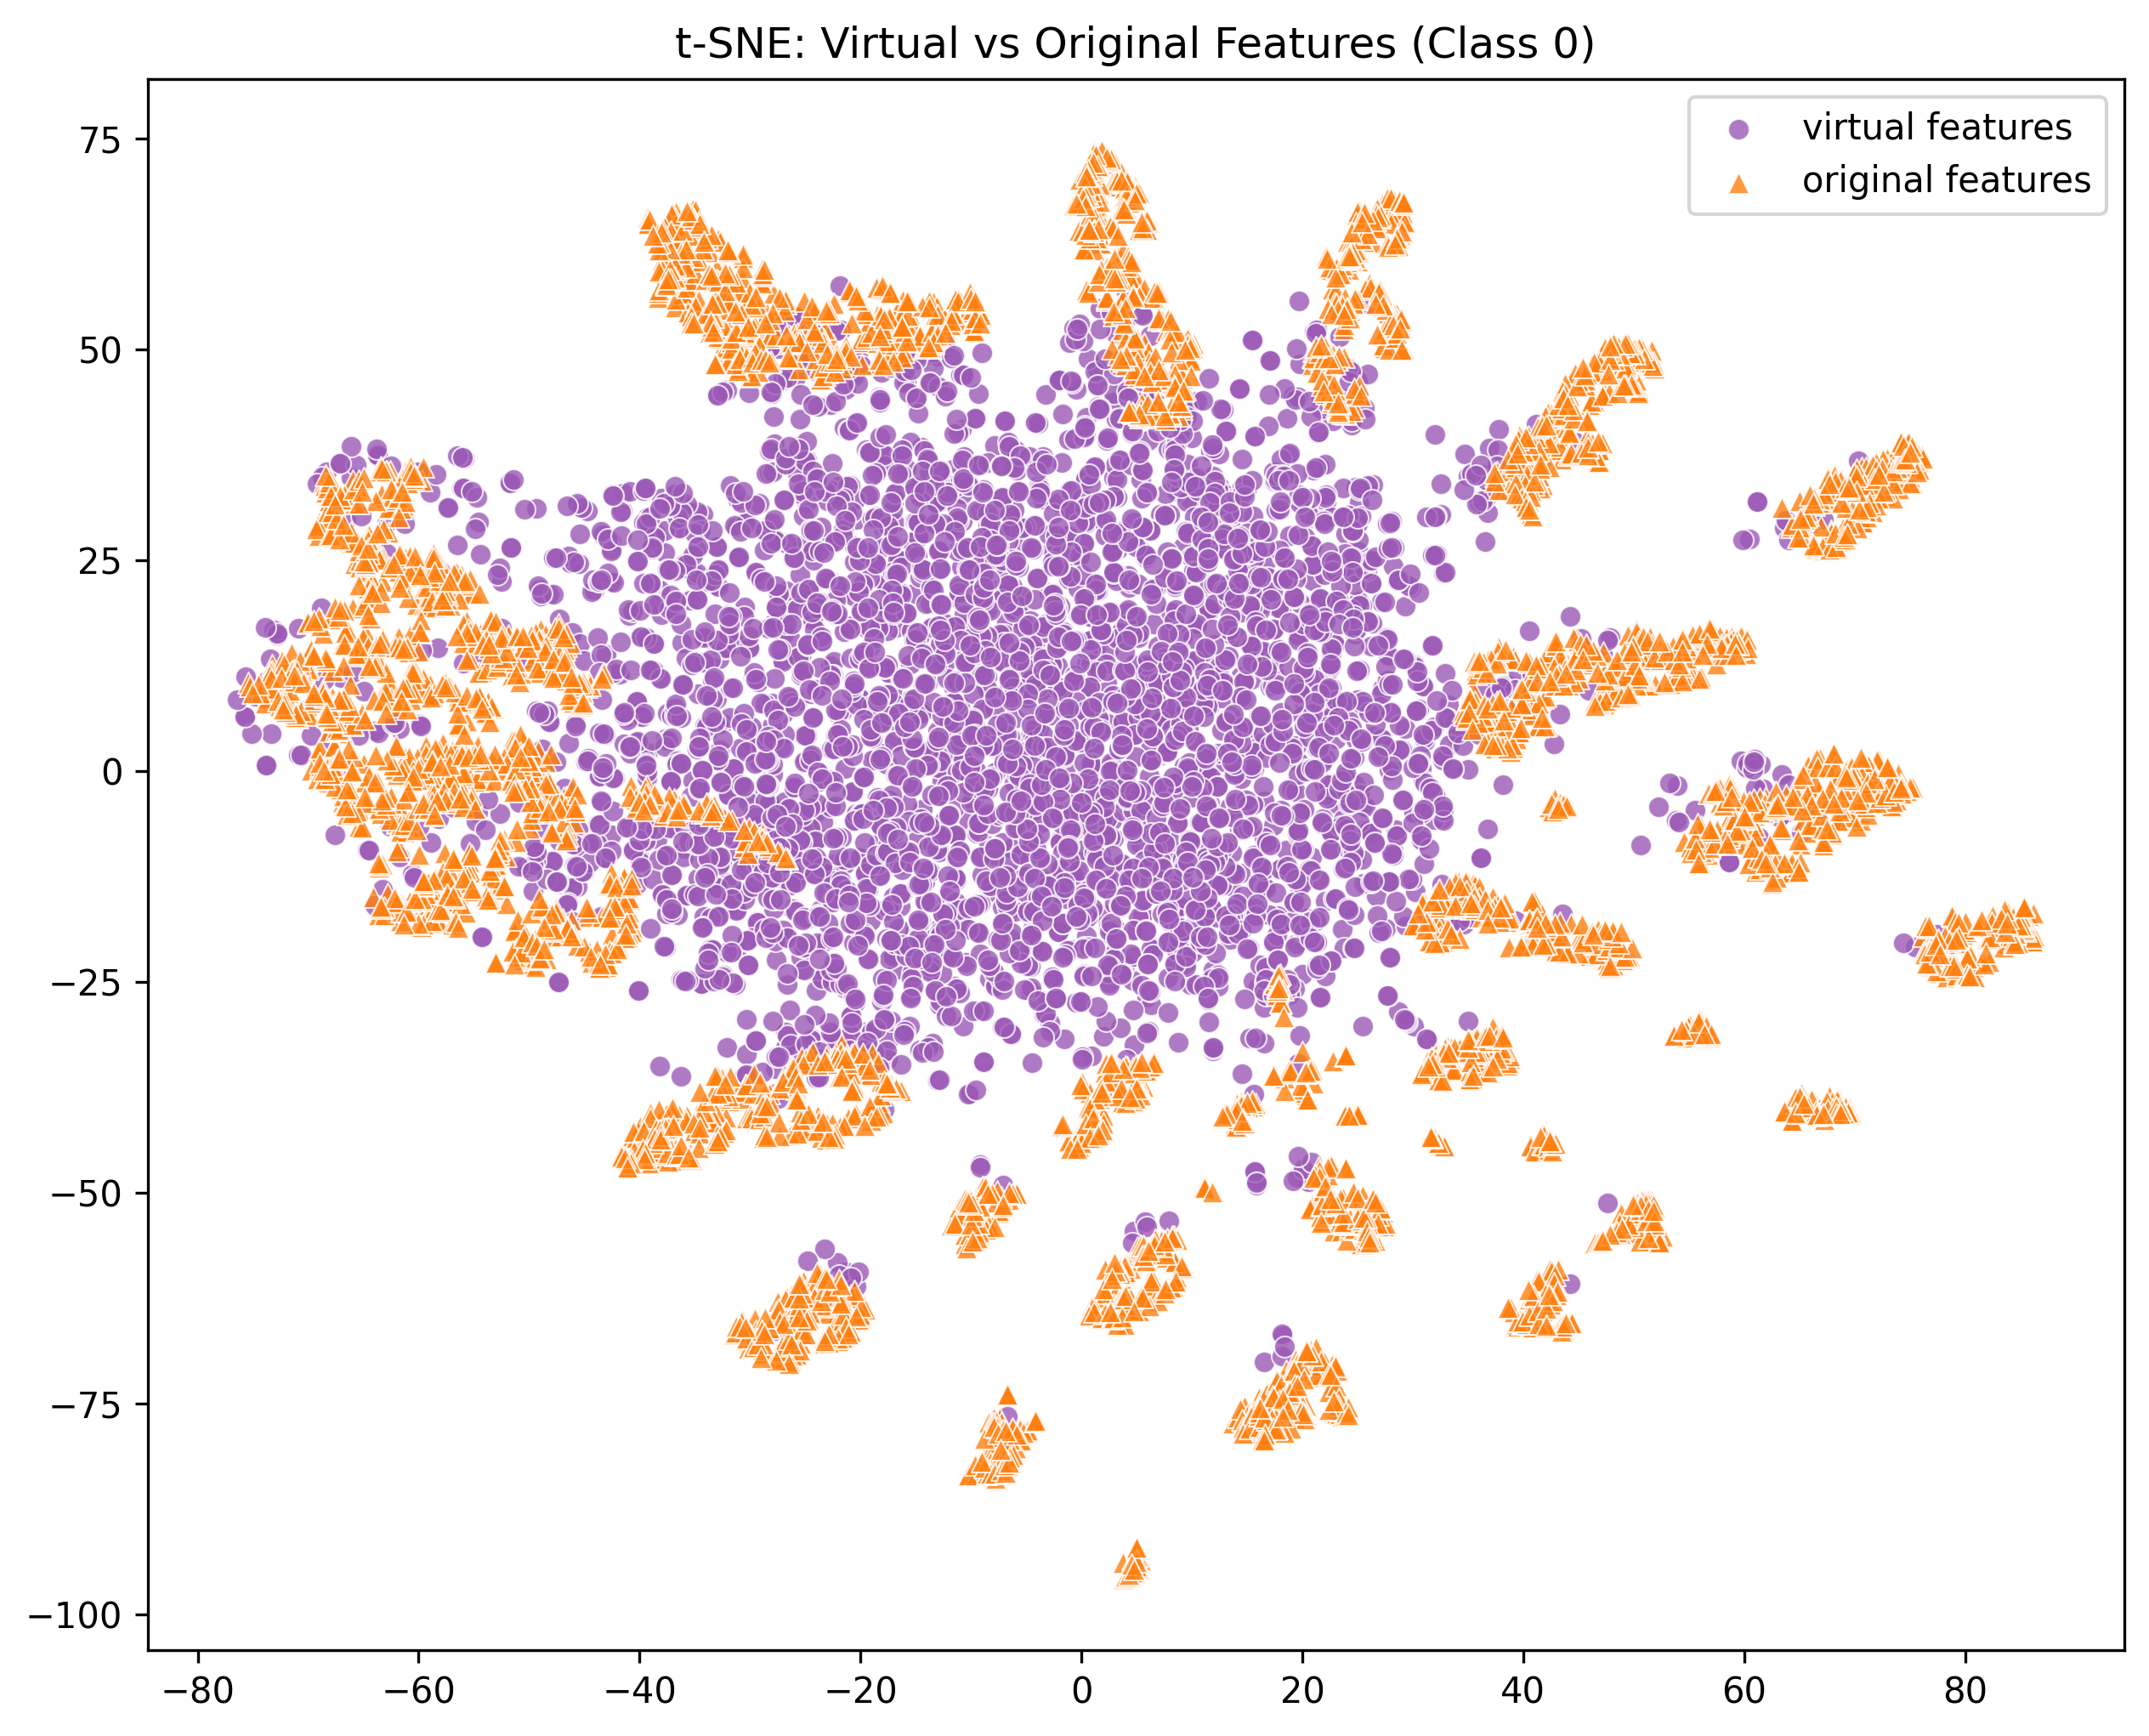
\includegraphics[width=0.8\linewidth]{imgs/tsne_class_0.png}
  \caption{After the first global round of training, the t-SNE visualization of virtual features and original features on FashionMNIST.}
  \label{tsne_class_0}
\end{figure}

\begin{figure*}[h]
    \centering
    \includegraphics[width=1\linewidth]{imgs/structure.png}
    \caption{General structure of the proposed semi-asynchronous energy-efficient federated prototype learning method}
    \label{fig:structure}
\end{figure*}

% \subsection{Details of Algorithm}

% The following is the algorithm.
\begin{breakablealgorithm}
  \caption{Semi-Asynchronous Energy-Efficient Federated Prototype learning for Client-Edge-Cloud Architectures}
  \begin{algorithmic}[1]
    % \State \textbf{Input: nothing}
    % \State \textbf{Output: nothing}

    \Procedure{cloud server executes}{}
    % \State Initialize global prototype set \( \bar{C}\) for all classes and weights for clients with heterogeneous models.
    \State Initialize weights for clients with heterogeneous models.
    \State All edge servers execute in parallel.
    \For{$t = 1, \dots, T$}
    \State Clear the buffer \(B\)

    \While{$B$ is not full} \Comment{Async process}
    \State Receive a triple \( (\mu^{l,edge}, \Sigma^{l,edge},\mathcal{N}^{l,edge}) \) from one edge server.
    \State Fill \( B \) with the received triple.
    \EndWhile
    \State \( \bar{C}, G \gets \text{CloudUpdate}(B) \)
    \State Send \( \bar{C}, G \) to edge servers participating on the current global aggregation.
    \State These edge servers re-execute.
    \EndFor
    \EndProcedure

    \Procedure{edge server executes}{}
    \State Receive \( \bar{C}, G \) from the cloud server
    \State Choose a set of clients $S^l$ to train in parallel.
    % \For{$e = 1, \dots, E$} \Comment{E now is static 1}
    \State Send \( \bar{C}, G \) to client \( i \in S^{l} \)
    \For{each client \( i \) in parallel}
    \State \( \textbf{ClientUpdate}(i, \bar{C}, G) \)
    \State Receive a triple \((\mu^{l,client}_i,\Sigma^{l,client}_i,\mathcal{N}^{l,client}_i)\)
    \EndFor \Comment{Wait for all clients}
    \State \( \textbf{EdgeAggregate}(\{ (\mu^{l,client}_i,\Sigma^{l,client}_i,\mathcal{N}^{l,client}_i) \}_{i \in S^{l}}) \)
    % \State \( \bar{C} \gets \text{EdgeUpdate}(\bar{C}, C^l) \) \Comment{not used now}
    % \EndFor
    \State Send a triple \( (\mu^{l,edge}, \Sigma^{l,edge},\mathcal{N}^{l,edge}) \) to the cloud server
    \EndProcedure
%   \end{algorithmic}
% \end{breakablealgorithm}

% % \newpage  % 强制换页

% \begin{breakablealgorithm}
%   \caption{Hierarchical Federated Prototype Learning -Part 2}
%   \begin{algorithmic}[1]
    \Procedure{CloudUpdate}{B}
    \State \( (\mu^{l,stored}, \Sigma^{l,stored},\mathcal{N}^{l,stored}) \gets (\mu^{l,edge}, \Sigma^{l,edge},\mathcal{N}^{l,edge})\quad\text{for}\quad l \in B \)
    \For{$j = 1, \dots, J$}
    \State \( \mathcal{N}_j = \sum_{l=1}^{L}\mathcal{N}^{l,stored}_{j} \)
    \State \( \text{Compute}\quad\mu_j,\Sigma_j\quad\text{by Eq. \ref{cloud mean},\ref{cloud covariance}}.  \)
    \EndFor
    \State Define $\mu$ as the global prototypes $\bar{C}$.
    \State Generate features \(X \sim \mathcal{N}(\mu, \Sigma)\) using the multivariate normal distribution.
    \State Use the virtual features \(X\) to train the global classifier \( G \).
    % \State Use adaptive-margin-enhanced contrastive learning to transform  $\bar{C}$ into $\bar{C}$
    \State \Return \( \bar{C}, G \)
    \EndProcedure
    
    \Procedure{EdgeAggregate}{$l, \{ (\mu^{l,client}_i, \Sigma^{l,client}_i,\mathcal{N}^{l,client}_i) \}_{i \in S^l}$}
    \State \( (\mu^{l,stored}_i, \Sigma^{l,stored}_i,\mathcal{N}^{l,stored}_i) \gets (\mu^{l,client}_i, \Sigma^{l,client}_i,\mathcal{N}^{l,client}_i)\quad\text{for}\quad i \in S^l \)
    \For{$j = 1, \dots, J$}
    \State \( \mathcal{N}^{l,edge}_j = \sum_{i=1}^{N^l}\mathcal{N}^{stored}_{i,j} \)
    \State \( \text{Compute}\quad\mu^{l,edge}_j,\Sigma^{l,edge}_j\quad\text{by Eq.\ref{edge mean},\ref{edge covariance}}.  \)
    \EndFor
    \State \Return \( (\mu^{l,edge}, \Sigma^{l,edge},\mathcal{N}^{l,edge}) \)
    \EndProcedure

    \Procedure{ClientUpdate}{$i, \bar{C}, G$}
    \State Receive \( \bar{C}, G \) from the edge server
    \State Only update one round and waiting for synchronization.
    \State Utilize the longest epoch training time to determine the operating frequency for subsequent rounds.
    \For{$e=1, \dots, E-1$}
    \State Scale the operating frequency.
    \For{batch (\(x,y\)) $\in$ \(D_i\)}
    \State Compute client prototypes by Eq.\ref{client prototype formula}.
    \State Compute loss by Eq. \ref{SAE loss function} using client prototypes and the global classifier $G$.
    \State Update client model according to the loss.
    \EndFor
    \EndFor
    \State Compute the mean $\mu^{l,client}_{i,j}$ and the covariance matrix  $\Sigma^{l,client}_{i,j}$ for features of each class 
    \Comment{Here, $\mu^{l,client}_{i,j}$ can be regarded as the prototype of class $j$ on the $i$-th client }
    \State \Return \( (\mu^{l,client}_i, \Sigma^{l,client}_i,\mathcal{N}^{l,client}_i) \)
    \EndProcedure
  \end{algorithmic}
\end{breakablealgorithm}

\section{Experiments}
\subsection{Setup}
\subsubsection{Datasets and algorithm implement}
We evaluate three popular benchmark datasets, including MNIST\cite{lecun1998mnist}, FashionMNIST\cite{xiao2017fashion}, and CIFAR-10\cite{krizhevsky2009learningcifar10}.  The client datasets are partitioned into training and testing sets in a 3:1 ratio.

For the implementation of the algorithm architecture, we extend the codebase of \cite{zhang2023pfllib}, adding a side for edge servers. In our setting, we simulate a cluster consisting of one cloud server, 10 edge servers, and 4 clients per edge server, with a client participation rate consistently set to 1. The number of local epochs is set to 5 and the number of global rounds is set to 200 for all experiments unless explicitly specified. To accelerate convergence and improve stability, we appropriately increase the batch size to 256, set the learning rate to 0.06, and configure the client training momentum of the SGD optimizer to 0.8.

For hyperparameter settings, we consistently set the importance weight $\lambda$ to 1, as reported in FedProto to achieve the highest test accuracy.  Additionally, we conduct comparative experiments by varying different $\gamma$ values. 
\subsubsection{Baselines}
We compared the proposed algorithm with several popular FL methods for heterogeneous models, including FedProto\cite{tan_fedproto_2021}, FedTGP\cite{zhang_fedtgp_2024}, FedGen\cite{zhu_data-free_fedgen_2021} , and  FedGH\cite{yi_fedgh_2023}.
\subsubsection{Statistical heterogeneity}
We conducted experiments following the practical statistical settings described in \cite{zhang_fedtgp_2024,li2021mode_moon}, and achieve the non-IID dataset partitioning using a Dirichlet distribution. Specifically, we sample \( q_j \sim Dir(\alpha) \) and allocate the proportion \( q_{i,j} \) of instances belonging to class \( j \) to client \( i \), where \( Dir(\alpha) \) denotes a Dirichlet distribution with parameter \(\alpha\). This partitioning scheme allows each client to possess relatively more data samples in certain classes while having fewer or no samples in most other classes.
\subsubsection{Model heterogeneity}
We evaluate the model heterogeneity using eight distinct types of feature extractors, as the same as   \cite{zhang_fedtgp_2024}. For MNIST and FashionMNIST,  the model group includes eight distinct convolutional neural network architectures, which are composed of varying combinations of one or two convolutional layers, followed by pooling layers, and up to three fully connected layers with dimensions selected from 512 and 1024. For CIFAR-10, the model group is consistent with \cite{zhang_fedtgp_2024}, including 4-layer CNN, GoogleNet, MobileNet v2, ResNet18, ResNet34, ResNet50, ResNet101, and ResNet152.

\subsubsection{Environment}
Accuracy tests are conducted using a machine equipped with 12 Intel(R) Xeon(R) Silver 4214R CPUs, an NVIDIA 3080 Ti GPU, and Ubuntu 22.04 LTS.

Edge devices are typically resource-constrained, operate under limited power availability, and are equipped with low performance computing and storage capabilities \cite{jiang2020energy}. To verify the energy saving effect in the real environment, FashionMNIST and MNIST are tested on NVIDIA Jetson TX2, which has a 6-core ARM CPU and 8GB DDR4 memory. The CPU frequency of Jetson TX2 range spans from 345,600 Hz to 2,035,200 Hz, with a total of 12 discrete frequency values. We utilize the interfaces provided in the NVIDIA documentation to monitor real-time power consumption and scale CPU frequencies.


\subsection{Accuracy of Methods}
As shown in the Table. \ref{PC_test}, FedSAE achieves the best performance. In scenarios with high model heterogeneity and a large number of clients, improving accuracy is particularly challenging. During training, FedSAE not only brings difficult-to-classify samples closer to the global prototype but also makes the inter-class distances more compact, as illustrated by Fig. \ref{exp_three_tsne}. FedProto shows a suboptimal clustering effect for prototypes, with the averaged prototypes of some clients exhibiting dispersed distributions that do not converge toward the global prototype. FedTGP effectively increases the inter-class distance, and the prototype aggregation is better than that of FedProto, but its accuracy is lower.

To illustrate again, the hyperparameter $\gamma$ determines the contribution of the global classifier to the loss during local training. When $\gamma=1$, the global classifier completely replaces the local classifier for training. For MNIST and FashionMNIST, where client models are relatively simple, appropriately tuning the value of $\gamma$ can balance the contributions of the global and local classifiers, thereby improving training performance. For CIFAR-10, $\gamma=1$ achieves the best performance under various data distributions. We attribute this to the higher model complexity, where relying entirely on the global classifier during training enables more effective adaptation to diverse data distributions.

As shown in Fig. \ref{Cifar10_dir_03_Model_loss}, it can be observed that, except for FedTGP, the loss for other methods stabilizes as training converges. We follow the contrastive learning parameter settings for the cloud server as described in \cite{zhang_fedtgp_2024}, but FedTGP struggles to converge with a larger batch size and requires appropriately tuned hyperparameters to achieve better performance. FedGH fails to train successfully on CIFAR-10. We suppose that this is due to the global classification head being trained solely on the averaged prototypes from clients, resulting in a significant mismatch between the local and global classification heads. Additionally, the lack of regularization constraints for local training exacerbates this discrepancy, leading to gradient explosion.




\begin{table*}[ht]
    \centering
    % \caption{The number of Edge servers is 10, 4 clients per edge server. Global rounds are set to 200, local epochs are set to 5, batchsize is 256, feature dimension is 512, local learning rate is 0.06, momentum is 0.8, \(\lambda\) is 1. Dirichlet distribution with a concentration parameter is $\alpha$. The buffer size of fedsae matches the number of edge servers.}
    \caption{The test accuracy on three datasets. The buffer size of FedSAE is equal to the number of edge servers.}
    \label{PC_test}
    \begin{tabular}{c c|c|c|c|c}
    \hline
    & & \multicolumn{2}{c|}{$\alpha = 0.1$}  & \multicolumn{2}{c}{$\alpha = 0.3$}\\
    \hline
    \textbf{Datasets} & \textbf{Methods} & \textbf{Prototype Acc(\%)} & \textbf{Model Acc(\%)} & \textbf{Prototype Acc(\%)} & \textbf{Model Acc(\%)} \\
    \hline
    \multirow{9}{*}{MNIST}
    & FedSAE($\gamma=1$) & \textbf{99.25} & 99.23 & 98.03 & 98.05  \\
    & FedSAE($\gamma=0.7$) & \textbf{99.25} & 99.23 & \textbf{98.08} & \textbf{98.08}  \\
    & FedSAE($\gamma=0.5$) & 99.24 & \textbf{99.24} & 98.04 & 98.06  \\
    & FedSAE($\gamma=0.2$) & 99.24 & 99.22 & 98.02 & 98.01  \\
    & Local Train & - & 98.97 & - & 97.31  \\
     & FedProto(AAAI'22) & 99.10 & 99.10 & 97.96 & 97.84 \\
     & FedTGP(AAAI'24) & 98.76 & 99.09 & 97.51 & 97.93 \\
     & FedGH(ACM MM'23) & - & 98.98 & - & 97.46 \\
     & FedGen(ICML'21) & - & 99.00 & - & 97.41 \\
    \hline
    \multirow{9}{*}{\makecell{Fashion\\ MNIST}} 
    & FedSAE($\gamma=1$) & 97.57 & 97.53 & 93.36 & 93.38 \\
    & FedSAE($\gamma=0.7$) & \textbf{97.62} & 97.55 & 93.30 & 93.41  \\
    & FedSAE($\gamma=0.5$) & 97.54 & \textbf{97.56} & \textbf{93.41} & \textbf{93.42}  \\
    & FedSAE($\gamma=0.2$) & 97.54  & 97.55 & 93.27 & 93.39  \\
    & Local Train & - & 97.15 & - & 92.56  \\
     & FedProto(AAAI'22) & 97.48 & 97.47 & 93.10 & 93.13 \\
     & FedTGP(AAAI'24) & \ding{55} & \ding{55} & \ding{55} & \ding{55} \\
     & FedGH(ACM MM'23) & - & 97.21(\ding{55}) & - & 92.51 \\
     & FedGen(ICML'21) & - & 97.34& - & 92.63\\
    \hline
    \multirow{9}{*}{CIFAR-10} 
    & FedSAE($\gamma=1$) & \textbf{82.06} & \textbf{82.08} & \textbf{67.27} & 67.22 \\
    & FedSAE($\gamma=0.7$) & 81.81 & 81.92 & 67.24 & \textbf{67.23} \\
    & FedSAE($\gamma=0.5$) & 81.62 & 81.60 & 67.11 & 67.01 \\
    & FedSAE($\gamma=0.2$) & 81.60 & 81.68 & 66.57 & 66.49 \\
    & Local Train & - & 81.06 & - & 65.97 \\
     & FedProto(AAAI'22) & 81.04 & 81.88 & 66.13 & 66.32 \\
     & FedTGP(AAAI'24) & 79.92 & 80.96 & 66.27 & 66.07 \\
     & FedGH(ACM MM'23) & - & \ding{55} & - & \ding{55} \\
     & FedGen(ICML'21) & - & 81.48 & - & 65.85\\
    \hline
    \end{tabular}
\end{table*}

\begin{figure}[htbp]
    \centering
    \includegraphics[width=0.96\linewidth]{imgs/Cifar10_dir_03_Model_loss.png}
    \caption{The training loss on CIFAR-10 with $\alpha=1$}
    \label{Cifar10_dir_03_Model_loss}
\end{figure}


\begin{figure*}[htbp]
    \centering
    % 子图1
    \subfloat[FedProto]{%
        \includegraphics[width=0.3\linewidth]{imgs/FedProto_tsne_agg_epoch_200_fd512.png}
        \label{FedProto_tsne_agg_epoch_200_fd512}
    }
    % 子图2
    \subfloat[FedSAE($\gamma=1$)]{%
        \includegraphics[width=0.3\textwidth]{imgs/FedSAE_gamma1_bf10_tsne_agg_epoch_200_fd512.png}
        \label{FedSAE_gamma1_bf10_tsne_agg_epoch_200_fd512}
    }
    \subfloat[FedTGP]{%
        \includegraphics[width=0.3\linewidth]{imgs/FedTGP_tsne_agg_epoch_200_fd512.png}
        \label{FedTGP_tsne_agg_epoch_200_fd512}
    }

    \caption{After 200 global rounds, the t-SNE visualization of aggregated prototypes generated by different methods on CIFAR-10. The experimental settings is consistent with Table \ref{PC_test}, and Dirichlet distribution parameter $\alpha=0.3$.}
    \label{exp_three_tsne}
\end{figure*}

\subsection{Energy Efficiency Experiment}
The size of the covariance matrix is proportional to the square of the dimension of the feature vectors. To reduce communication overhead, the dimension of the feature vectors is set to 64. Following the experimental setup in [citation needed], the communication time between the edge server and the cloud server is assumed to be 10 times that between the clients and the edge server. The communication time is calculated using Shannon's formula.

\begin{table*}[ht]
    \centering
    \caption{The number of Edge servers is 10, 4 clients per edge server and Buffer Size (BS) of FedSAE: $\{1, 4, 7\}$. \\ Other Experimental Settings is Consistent with Table \ref{PC_test}, and Dirichlet distribution parameter $\alpha=0.3$.}
    \begin{tabular}{|c|c|c|c|c|c|c|}
    \hline
    \textbf{Datasets} & \textbf{Methods} & \textbf{Global Time(s)} & \textbf{Train Time(s)} & \textbf{Prototype Acc(\%)} & \textbf{Model Acc(\%)} & \textbf{Energy (kJ)}\\  
    \hline
    \multirow{5}{*}{MNIST} 
    & FedSAE(Full~buffer~size) &  &  &  & &  \\
    & FedSAE($BS=7$) &  &  &  & &  \\
    & FedSAE($BS=4$) &  &  &  &  &  \\
    & FedSAE($BS=1$) &  &  &  &  &  \\
    % & Local Train &  &  &  &  &  \\
    & FedProto &  &  &  &  & \\
    & FedProto + DVFS &  &  &  &  & \\
    \hline
    \multirow{5}{*}{\makecell{Fashion\\ MNIST}} 
    & FedSAE(Full~buffer~size) &  &  &  & &  \\
    & FedSAE($BS=7$) &  &  &  & &  \\
    & FedSAE($BS=4$) &  &  &  &  &  \\
    & FedSAE($BS=1$) &  &  &  &  &  \\
    % & Local Train &  &  &  &  &  \\
    & FedProto &  &  &  &  & \\
    & FedProto + DVFS &  &  &  &  & \\
    \hline
    \end{tabular}
\end{table*}

\begin{table}[ht]
    \centering
    \caption{Test accuracies(\%) on CIFAR-10 with different feature dimensions. The number of Edge servers is 10, 4 clients per edge server. the $\gamma$ of fedsae is 1.}
    \begin{tabular}{|c|c|c|c|c|}
    \hline
    \textbf{Methods} & $Dim$\newline =64  & $Dim$=256 & $Dim$=1024 \\
    \hline
    Local Train & 66.16 & 66.33 & 65.31 \\
    FedSAE & 67.24/67.40 & 66.87/66.95 & \textbf{65.73/65.68} \\
    FedProto & 66.90/67.00 & 67.27/67.17 & 64.96/65.13 \\
    FedTGP & \textbf{67.83/67.47} & \textbf{67.45/67.23} & 64.30/65.20\\
    % FedGH &  &  & \\
    FedGen & 66.39 & 66.66 & 65.81 \\
    \hline
    \end{tabular}
\end{table}



\subsection{Communication Cost}

\section{Conclusion}

\bibliography{SAE} 
\bibliographystyle{IEEEtran}


\onecolumn

\section{Derivation of both Global Mean and Covariance}
\(k\) is the \(k\)-th client, \(l\) is the \(l\)-th edge server, \(c\) is the \(c\)-th class. \( N(c,k,l) \) is the number of samples of class \( c \) in the client \( k \) on the edge server \( l \). \( N(c,l) \) is the number of samples of class \( c \) in the edge server \( l \). \( N(c) \) is the number of samples of class \( c \) at the cloud server.

Mean and covariance of client:
\begin{equation}
\mathbf{\mu}_{c,k,l} = \frac{1}{N(c,k,l)} \sum_{i=1}^{N(c,k,l)} \mathbf{x}_{i,c,k,l}
\end{equation}
\begin{equation}
\mathbf{\Sigma}_{c,k,l} = \frac{1}{N(c,k,l)-1} \sum_{i=1}^{N(c,k,l)} \big( \mathbf{x}_{i,c,k,l} - \mathbf{\mu}_{c,k,l} \big) \big( \mathbf{x}_{i,c,k,l} - \mathbf{\mu}_{c,k,l} \big)^\top,
\end{equation}

Mean and covariance of edge:
\begin{equation}
  N(c,l) = \sum_{k=1}^K N(c,k,l).
\end{equation}
\begin{equation}
    \mathbf{\mu}_{c,l} = \frac{1}{N(c,l)} \sum_{k=1}^K N(c,k,l) \mathbf{\mu}_{c,k,l},
    \end{equation}
\begin{equation}
\mathbf{\Sigma}_{c,l} = \frac{1}{N(c,l)-1} \sum_{k=1}^K \Bigg[
\big( N(c,k,l)-1 \big) \mathbf{\Sigma}_{c,k,l} + N(c,k,l) \big( \mathbf{\mu}_{c,k,l} - \mathbf{\mu}_{c,l} \big) \big( \mathbf{\mu}_{c,k,l} - \mathbf{\mu}_{c,l} \big)^\top
\Bigg],
\end{equation}

Derivation of edge covariance:

Consider \( \mathbf{z}_{i,c,k,l} = \mathbf{x}_{i,c,k,l} - \mathbf{\mu}_{c,k,l} \) as the deviation of the sample from the local mean at the client \(k \). And \(\sum_{i=1}^{N(c,k,l)} \mathbf{z}_{i,c,k,l} = 0  \)

\begin{align*}
  \mathbf{\Sigma}_{c,l} &= \frac{1}{N(c,l)-1} \sum_{k=1}^K \sum_{i=1}^{N(c,k,l)} \big( \mathbf{x}_{i,c,k,l} - \mathbf{\mu}_{c,l} \big) \big( \mathbf{x}_{i,c,k,l} - \mathbf{\mu}_{c,l} \big)^\top \\
  &= \frac{1}{N(c,l)-1} \sum_{k=1}^K \sum_{i=1}^{N(c,k,l)} \left( \big( \mathbf{\mu}_{c,k,l} + \mathbf{z}_{i,c,k,l} - \mathbf{\mu}_{c,l} \big) \big( \mathbf{\mu}_{c,k,l} + \mathbf{z}_{i,c,k,l} - \mathbf{\mu}_{c,l} \big)^\top \right) \\
  &= \frac{1}{N(c,l)-1} \sum_{k=1}^K \sum_{i=1}^{N(c,k,l)} \Bigg[ \big( \mathbf{\mu}_{c,k,l} - \mathbf{\mu}_{c,l} \big) \big( \mathbf{\mu}_{c,k,l} - \mathbf{\mu}_{c,l} \big)^\top \\
  &\quad + \mathbf{z}_{i,c,k,l} \mathbf{z}_{i,c,k,l}^\top + \big( \mathbf{\mu}_{c,k,l} - \mathbf{\mu}_{c,l} \big) \mathbf{z}_{i,c,k,l}^\top + \mathbf{z}_{i,c,k,l} \big( \mathbf{\mu}_{c,k,l} - \mathbf{\mu}_{c,l} \big)^\top \Bigg] \\
  &= \frac{1}{N(c,l)-1} \sum_{k=1}^K \Bigg[ (N(c,k,l)-1) \mathbf{\Sigma}_{c,k,l} + N(c,k,l) \big( \mathbf{\mu}_{c,k,l} - \mathbf{\mu}_{c,l} \big) \big( \mathbf{\mu}_{c,k,l} - \mathbf{\mu}_{c,l} \big)^\top \Bigg]
\end{align*}

Mean and covariance of cloud:

First, use the decomposition:
\begin{equation}
\mathbf{x}_{i,c,k,l} - \mathbf{\mu}_c = \big( \mathbf{x}_{i,c,k,l} - \mathbf{\mu}_{c,l} \big) + \big( \mathbf{\mu}_{c,l} - \mathbf{\mu}_c \big),
\end{equation}

We substitute into the covariance definition:
\begin{align*}
\mathbf{\Sigma}_c 
&= \frac{1}{N(c)-1} \sum_{l=1}^L \sum_{k=1}^K \sum_{i=1}^{N(c,k,l)} 
\big( \mathbf{x}_{i,c,k,l} - \mathbf{\mu}_c \big) \nonumber \times 
\big( \mathbf{x}_{i,c,k,l} - \mathbf{\mu}_c \big)^\top \\ 
&= \frac{1}{N(c)-1} \sum_{l=1}^L \sum_{k=1}^K \sum_{i=1}^{N(c,k,l)} 
\Big[
\big( \mathbf{x}_{i,c,k,l} - \mathbf{\mu}_{c,l} \big) + \big( \mathbf{\mu}_{c,l} - \mathbf{\mu}_c \big)
\Big] \nonumber \\
&\qquad \times 
\Big[
\big( \mathbf{x}_{i,c,k,l} - \mathbf{\mu}_{c,l} \big) + \big( \mathbf{\mu}_{c,l} - \mathbf{\mu}_c \big)
\Big]^\top.
\end{align*}

Expanding the terms:
\begin{align}
\mathbf{\Sigma}_c &= \frac{1}{N(c)-1} \sum_{l=1}^L \sum_{k=1}^K \sum_{i=1}^{N(c,k,l)} 
\Big[
\mathbf{Z}_{i,c,k,l} \mathbf{Z}_{i,c,k,l}^\top + 
\mathbf{Z}_{i,c,k,l} \big( \mathbf{\mu}_{c,l} - \mathbf{\mu}_c \big)^\top \nonumber \\
&\qquad + 
\big( \mathbf{\mu}_{c,l} - \mathbf{\mu}_c \big) \mathbf{Z}_{i,c,k,l}^\top + 
\big( \mathbf{\mu}_{c,l} - \mathbf{\mu}_c \big) \big( \mathbf{\mu}_{c,l} - \mathbf{\mu}_c \big)^\top
\Big].
\end{align}

Here, \( \mathbf{Z}_{i,c,k,l} = \mathbf{x}_{i,c,k,l} - \mathbf{\mu}_{c,l} \) represents the deviation of local samples from their respective edge means.

Simplification of Cross Terms
The cross terms are:
\begin{equation}
\mathbf{Z}_{i,c,k,l} \big( \mathbf{\mu}_{c,l} - \mathbf{\mu}_c \big)^\top, \quad
\big( \mathbf{\mu}_{c,l} - \mathbf{\mu}_c \big) \mathbf{Z}_{i,c,k,l}^\top.
\end{equation}

Summing over all samples, these terms vanish because:
\begin{equation}
  \sum_{k=1}^K \sum_{i=1}^{N(c,k,l)} \mathbf{Z}_{i,c,k,l} = \mathbf{0}
\end{equation}

Consider the summation of deviations for client \( k \) at edge \( l \):
\begin{align*}
\sum_{k=1}^K\sum_{i=1}^{N(c,k,l)} \mathbf{Z}_{i,c,k,l} &= \sum_{k=1}^K \sum_{i=1}^{N(c,k,l)} \big( \mathbf{x}_{i,c,k,l} - \mathbf{\mu}_{c,l} \big) \\
&= \sum_{k=1}^K\sum_{i=1}^{N(c,k,l)} \mathbf{x}_{i,c,k,l} - \sum_{k=1}^K\sum_{i=1}^{N(c,k,l)} \mathbf{\mu}_{c,l}. \\
&= \sum_{k=1}^K\sum_{i=1}^{N(c,k,l)} \mathbf{x}_{i,c,k,l} - \sum_{k=1}^K N(c,k,l) \mathbf{\mu}_{c,l} \\
&= \sum_{k=1}^K\sum_{i=1}^{N(c,k,l)} \mathbf{x}_{i,c,k,l} - \sum_{k=1}^K\frac{N(c,k,l)}{N(c,l)} \sum_{k=1}^K \sum_{i=1}^{N(c,k,l)} \mathbf{x}_{i,c,k,l} \\
&= 0
\end{align*}



Final Formula
The cloud-level covariance reduces to:
\begin{align}
\mathbf{\Sigma}_c &= \frac{1}{N(c)-1} \Bigg[
\sum_{l=1}^L \sum_{k=1}^K \sum_{i=1}^{N(c,k,l)} \mathbf{Z}_{i,c,k,l} \mathbf{Z}_{i,c,k,l}^\top + 
\sum_{l=1}^L N(c,l) \big( \mathbf{\mu}_{c,l} - \mathbf{\mu}_c \big) \big( \mathbf{\mu}_{c,l} - \mathbf{\mu}_c \big)^\top
\Bigg] \nonumber \\
&= \frac{1}{N(c)-1} \Bigg[
\sum_{l=1}^L (N(c,l)-1) \mathbf{\Sigma}_{c,l} + 
\sum_{l=1}^L N(c,l) \big( \mathbf{\mu}_{c,l} - \mathbf{\mu}_c \big) \big( \mathbf{\mu}_{c,l} - \mathbf{\mu}_c \big)^\top
\Bigg].
\end{align}


\section{Features of test dataset}

\begin{figure*}[htbp]
    \centering
    % % 子图1
    % \subfloat[Average Prototypes of FedSAE($\gamma$=1)]{%
    %     \includegraphics[width=0.45\linewidth]{imgs/test_umap_FedSAE_visualization_protos.png}
    %     \label{test_umap_FedSAE_visualization_protos}
    % }
    % % \hfill
    % % 子图2
    % \subfloat[Average Prototypes of  FedProto]{%
    %     \includegraphics[width=0.45\linewidth]{imgs/test_umap_FedSAE_visualization_protos.png}
    %     \label{test_umap_FedSAE_visualization_protos}
    % }


    \subfloat[Features of FedSAE($\gamma$=1)]{%
        \includegraphics[width=0.45\linewidth]{imgs/onlytrue_umap_FedSAE_visualization.png}
        \label{onlytrue_umap_FedSAE_visualization}
    }
    % \hfill
    % 子图2
    \subfloat[Features of FedProto]{%
        \includegraphics[width=0.45\linewidth]{imgs/onlytrue_umap_FedProto_visualization.png}
        \label{onlytrue_umap_FedProto_visualization}
    }

    \caption{After 200 global rounds, the UMAP visualization\cite{mcinnes2018umap-software} of features of correctly classified samples on CIFAR-10 where $\alpha$=0.1, local train epochs is 5, and the dimension of hidden features (prototypes) is 512.}
    \label{UMAP}
\end{figure*}

\end{document}


